%  LaTeX support: latex@mdpi.com 
%  For support, please attach all files needed for compiling as well as the log file, and specify your operating system, LaTeX version, and LaTeX editor.

%=================================================================
\documentclass[journal,article,submit,pdftex,moreauthors]{Definitions/mdpi} 


% MDPI internal commands - do not modify
\firstpage{1} 
\makeatletter 
\setcounter{page}{\@firstpage} 
\makeatother
\pubvolume{1}
\issuenum{1}
\articlenumber{0}
\pubyear{2024}
\copyrightyear{2024}
%\externaleditor{Academic Editor: Firstname Lastname}
\datereceived{ } 
\daterevised{ } % Comment out if no revised date
\dateaccepted{ } 
\datepublished{ } 
%\datecorrected{} % For corrected papers: "Corrected: XXX" date in the original paper.
%\dateretracted{} % For corrected papers: "Retracted: XXX" date in the original paper.
\hreflink{https://doi.org/} % If needed use \linebreak
%\doinum{}
%\pdfoutput=1 % Uncommented for upload to arXiv.org
%\CorrStatement{yes}  % For updates




% Full title of the paper (Capitalized)
\Title{Improving the  
Giant Armadillo Optimization method}

% MDPI internal command: Title for citation in the left column
\TitleCitation{
Improving the  
Giant Armadillo Optimization method }

\Author{Glykeria Kyrou $^{1}$, Vasileios Charilogis$^{2}$, Ioannis G.Tsoulos$^{3}$}
\AuthorNames{Glykeria Kyrou, Ioannis G.Tsoulos}
\AuthorCitation{Kyrou, G.; Charilogis, V.; Tsoulos, I.G.}
\address{%
$^{1}$ \quad Department of Informatics and Telecommunications, University of Ioannina; mailto:g.kyrou@uoi.gr\\

$^{2}$ \quad Department of Informatics and Telecommunications, University of Ioannina; mailto:v.charilog@uoi.gr\\
$^{3}$ \quad Department of Informatics and Telecommunications, University of Ioannina; itsoulos@uoi.gr}

\corres{Correspondence: itsoulos@uoi.gr}
\abstract{Global optimization is widely adopted nowadays in a variety of practical and scientific problems. In this context, a group of techniques that is widely used is that of evolutionary techniques. A relatively new evolutionary technique in this direction is that of Giant Armadillo Optimization, which is based on the hunting strategy of giant armadillos. In this paper, a number of modifications to this technique are proposed, such as the periodic application of a local minimization method as well as the use of modern termination techniques based on statistical observations. The proposed modifications have been tested on a wide - series test functions, available from the relevant literature and it was compared against other evolutionary methods.
}

% Keywords
\keyword{Global optimization; evolutionary methods; stochastic methods} 



\begin{document}


\section{Introduction}
Global optimization targets to discover the global minimum of an optimization problem by searching in the domain range of this problem. Typically,  a global optimization method aims to discover the global minimum of  a continuous function $f:S\rightarrow R,S\subset R^{n}$\textbf{
} and hence the global optimization problem is formulated as:
\begin{equation}
x^{*}=\mbox{arg}\min_{x\in S}f(x).\label{eq:eq1}
\end{equation}
The set $S$ is defined as:\textbf{ 
\[
S=\left[a_{1},b_{1}\right]\otimes\left[a_{2},b_{2}\right]\otimes\ldots\left[a_{n},b_{n}\right]
\]
}
The vectors $a$ and $b$  stand for the left and right bounds respectively
for the point $x$.  A  review of the optimization procedure can be found in the paper of Rothlauf \cite{rothlauf2011optimization}. Global optimization refers to techniques that seek the optimal solution to a problem, mainly using traditional mathematical methods, for example methods that try to locate either maxima or minima \cite{horst2000introduction,weise2009global,ovelade2021ebola}. Every optimization problem contains its decision variables, a possible series of constraints and the definition of the objective function\cite{deb2016multi}.  Every optimization method targets to discover appropriate values for the decision variables, in order to minimize the objective function. The optimization methods are commonly  divided into deterministic and stochastic approaches \cite{liberti2005comparison}. The techniques used in most cases for the first category are the interval methods \cite{interval1, interval2}. In interval methods, the set $S$ is divided  through a number of iterations into  subareas that may contain the global minimum using some criteria. On the other hand, stochastic optimization methods are used in the majority of cases, because they can be programmed faster than deterministic ones
 and they do not depend on  any previously defined information about the objective function. Such techniques may include Controlled Random Search methods \cite{crs1,crs2, crs3}, Simulated Annealing methods \cite{siman1,siman2}, Clustering methods \cite{clustering1, clustering2, clustering3} etc.  Systematic reviews of stochastic methods can be located  in the paper of Pardalos et al \cite{pardalos2000recent} or in the paper of Fouskakis et al \cite{fouskakis2002stochastic}. Also, due to the widespread use of parallel computing techniques, a series of methods have been presented that exploit such architectures \cite{msgpu1, msgpu2}.
\\
A group of stochastic programming techniques that have been proposed to tackle optimization problems are evolutionary techniques. These techniques are biological inspired, heuristic and population-based \cite{bartz2014evolutionary,simon2013evolutionary}.
Some techniques that belong to evolutionary techniques are for example Ant Colony Optimization methods \cite{aco1, aco2}, Genetic algorithms \cite{geneticReview,jamwal2019evolutionary,wang2020comparative}, Particle Swarm Optimization (PSO) methods \cite{psomajor,psoReview}, Differential Evolution techniques \cite{deprice,deReview}, evolutionary strategies \cite{asselmeyer1997evolutionary,arnold2002noisy}, evolutionary programming \cite{yao1999evolutionary},  genetic programming \cite{stephenson2003genetic}  etc. These methods have been with success in a series of practical problems from many fields, for example biology \cite{banga2008optimization,beites2015chassis}, physics \cite{hartmann2002optimization,hanuka2021physics}, chemistry \cite{ferreira2018multivariate,bechikh2014efficient}, agriculture \cite{ filip2020advanced,zhang2016integrated}, economics \cite{intriligator2002mathematical, dixit1990optimization}.

Metaheuristic algorithms from their appearance in the early 70s to the late 90s have seen significant developments.
Metaheuristic algorithms have gained much attention in solving difficult optimization problems and are paradigms of computational intelligence \cite{meta1,meta2,meta3}. Metaheuristic algorithms are grouped into four categories based on their behavior: evolutionary algorithms, algorithms based on considerations derived from physics,  algorithms based on swarms and human-based algorithms\cite{metadivide}.

Recently, Alsayyed et al \cite{alsayyed2023giant} introduced a new   bio-inspired  algorithm that belongs to the group of metaheuristic algorithms. This new algorithm is called  Giant Armadillo Optimization (GAO) and aims to replicate the behavior of giant armadillos in the real-world \cite{desbiez2021methods}. The new algorithm is based on the giant armadillo's hunting strategy of heading towards prey and digging termite mounds.

Owaid et al present a method \cite{owaid2024development} concerning the decision-making process in organizational and technical systems management problems, which  also uses giant armadillo agents. The article presents a method for maximizing decision-making capacity in organizational and technical systems using artificial intelligence. The research is based on giant armadillo agents that are trained with the help of artificial neural networks \cite{nn1,nn2} and in addition a genetic algorithm is used to select the best one.

The GAO optimizer can also be considered as a method based on Swarm Intelligence \cite{swarm_book}. Some of the reasons why methods based on Swarm Intelligence are used in optimization problems are their robustness, scalability as well as their flexibility. With the help of simple rules, simple reactive agents such as fish and birds exchange information with the basic purpose of finding an optimal solution \cite{swarm_overview1,swarm_overview2}.
This article focuses on enhancing the effectiveness and the speed of the  GAO algorithm by proposing some modifications and more specifically: 
\begin{itemize}
    \item  Application of  termination rules, that are based on asymptotic considerations and they are defined in the recent bibliography. This addition will achieve early termination of the method and will not waste computational time on iterations that do not yield a better estimate of the global minimum of the objective function.
    \item A periodic application of a local search procedure. By using local optimization, the local minima of the objective function will be found more efficiently, which will also lead to a faster discovery of the global minimum.

\end{itemize}
The current method was applied on a series of objective problems found in the  literature of global optimization and it is compared against an implemented Genetic Algorithm and a variant of the PSO technique.\\

The rest of this paper is divided into the following sections: in section \ref{sec:Method} the proposed modifications are fully described, in section \ref{sec:Results} the benchmark functions are listed accompanied by  the experimental results and finally in section \ref{sec:Conclusions} some conclusions and guidelines for future work are provided.

\section{The proposed method}\label{sec:Method}
The GAO algorithm is based on processes inspired by the nature and initially generates a population of candidate solutions, that are possible solutions of the objective problem. The GAO algorithm aims to evolve the population of solutions through iterative steps.  The algorithm has two major phases: the exploration phase, where the candidate solutions are updated with a process that mimics the attack of armadillos on termite mounds and the exploitation phase, where the solutions are updated similar to digging in termite mounds. The basic steps of the GAO algorithm are presented below:

\begin{enumerate}
   
\item \textbf{Initialization step}
\begin{itemize}
    \item  \textbf{Define}  as $N_c$ as number of armadillos in the population.
    \item  \textbf{Define} as $N_g$ the  number of allowed iterations.
    \item \textbf{Initialize} randomly the $N_c$ $g_i,\ i=1,\ldots,N_c$ armadillos in $S$.
    \item \textbf{Set} iter=0.
    \item  \textbf{Set} $p_l$ the local search rate.
\end{itemize}
\item \textbf{Evaluation step}
\begin{itemize}
  \item \textbf{For} $i=1,\ldots,N_c$ \textbf{do} Set 
  $f_i=f\left(g_i\right)$.
  \item  \textbf{endfor}
\end{itemize}
\item \textbf{Computation step} \label{enu:compu}
    \begin{itemize}
        \item \textbf{For} $i=1,\ldots,N_c$ \textbf{do}
        \begin{enumerate}
            \item \textbf{Phase 1}: Attack on termite mounds 
            \begin{itemize}
                \item Create a set that contains the termites as
                $\mbox{TM}_i=\left\{g_{k_i}: f_{k_i}<f_i\  \mbox{and}\  k_i\ne i \right\}$
                \item Select the termite mound $\mbox{STM}_i$ for armadillo $i$.
                \item  Create a new position $g^{\mbox{P1}}_i$ for the armadillo according to the formula: $g^{\mbox{P1}}_{i,j}=g_{i,j}+r_{i,j}\left( \mbox{STM}_{i,j}-I_{i,j}g_{i,j}\right)$ where $r_{i,j}$ are random numbers in $[0,1]$ and $I_{i,j}$ are random numbers in $[1,2]$ and $j=1,\ldots,n$
                \item Update the position of the armadillo $i$ according to:
                \[
                g_{i}=\begin{cases}
                \begin{array}{cc}
                    g_{i}^{\mbox{P1}},\  & f\left(g_{i}^{\mbox{P1}}\right)\le f_{i}\\
                    g_{i} & \mbox{otherwise}
                    \end{array}
                    \end{cases}\]
            \end{itemize}
            \item \textbf{Phase 2:} Digging in termite mounds 
            \begin{itemize}
                \item Create a new trial position
                \[
                  g^{\mbox{P2}}_{i,j}=g_{i,j}+(1-2r_{i,j})\frac{b_j-a_j}{\mbox{iter}}
                \] 
                where $r_{i,j}$ are random numbers in $[0,1]$.
                 \item Update the position of the armadillo $i$ according to:
                \[
                g_{i}=\begin{cases}
                \begin{array}{cc}
                    g_{i}^{\mbox{P2}},\  & f\left(g_{i}^{\mbox{P2}}\right)\le f_{i}\\
                    g_{i} & \mbox{otherwise}
                    \end{array}
                    \end{cases}\]
            \end{itemize}
            \item \textbf{Local search}. Pick a random number $r\in[0,1]$. If $r\le p_l$ then a local optimization algorithm is applied to  $g_i$.  Some local search procedures found in the  optimization literature are the  BFGS method \cite{bfgs}, the Steepest Descent  method \cite{stepestdescent},  the L-Bfgs method \cite{lbfgs} for large scaled optimization etc.  A BFGS modification proposed by Powell \cite{tolmin} was used in the current work as the local search optimizer. Using the  local optimization technique ensures that the outcome of the global optimization method will be one of the local minima of the objective function. This ensures maximum accuracy in the end result.
        \end{enumerate} 
        \item  \textbf{endfor}
    \end{itemize}


\item \textbf{Termination check step}
\begin{itemize}
  
 \item \textbf{Set} iter=iter+1. 

\item For the  valid termination of the method, two termination rules that have recently appeared in the literature are proposed here and they are based on  stochastic considerations. The first stopping rule will be called \textit{DoubleBox} in the conducted experiments and it was introduced in the work of Tsoulos in 2008 \cite{tsoulos2008modifications}. The steps for this termination rule have as follows:
\begin{enumerate}
    \item Define as $\sigma^{\mbox{iter}}$ the variance of located global miniumum at  iteration iter.
    \item Terminate when $\mbox{iter}\ge N_g\ \mbox{OR}\ \sigma^{\mbox{iter}} \le \frac{\sigma^{k_T}}{2} $
\end{enumerate} where $k_T$ is the iteration where a new better estimation for the global minimum was firstly found.\\
The second termination rule was introduced in the work of Charilogis et al \cite{ipso}
and will be called \textit{Similarity} in the experiments. 
In \textit{Similarity} stopping rule, at every iteration \ensuremath{k},
the absolute difference between the current located global minimum $f_{min}^{(k)}$
and the previous best value $f_{min}^{(k+1)}$ is calculated:
\begin{center}
\[
\left|f_{\mbox{min}}^{(k)}-f_{\mbox{min}}^{(k-1)}\right|
\]
\par\end{center}

If this difference is zero for a predefined number of consecutive
generations $N_{k}$, the method terminates.

\item If the termination criteria are not hold then goto step \ref{enu:compu}.
\end{itemize}

\end{enumerate}
The steps of the proposed method are also outlined in Figure \ref{fig:diagram}.
\begin{figure}[H]

\hspace{-5pt}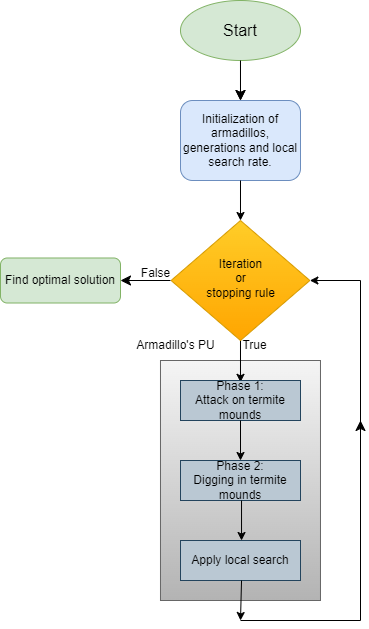
\includegraphics[scale=0.75]{armadillo_diagram.png}
\caption{A schematic repreantation of the current method. \label{fig:diagram}}
\end{figure}

\section{Experiments}\label{sec:Results}
This section will begin by detailing the functions that will be used in the experiments. These functions are widespread in the modern global optimization literature and have been used in many research works. Next, the experiments performed using the current method will be presented and a comparison will be made with methods that are commonly used in the literature of global optimization.

\subsection{Experimental functions}
The functions used in the conducted experiments can be found in the related literature \cite{ali2005numerical,floudas2013handbook}. The definitions for the
functions are listed subsequently.
\begin{itemize}

\item \textbf{Bf1} function, defined as:
\end{itemize}
\[
f(x)=x_{1}^{2}+2x_{2}^{2}-\frac{3}{10}\cos\left(3\pi x_{1}\right)-\frac{4}{10}\cos\left(4\pi x_{2}\right)+\frac{7}{10}
\]
\begin{itemize}
\item \textbf{Bf2} function, defined as:
\[
f(x)=x_{1}^{2}+2x_{2}^{2}-\frac{3}{10}\cos\left(3\pi x_{1}\right)\cos\left(4\pi x_{2}\right)+\frac{3}{10}
\]
\item \textbf{Branin} function, defined as: $f(x)=\left(x_{2}-\frac{5.1}{4\pi^{2}}x_{1}^{2}+\frac{5}{\pi}x_{1}-6\right)^{2}+10\left(1-\frac{1}{8\pi}\right)\cos(x_{1})+10$.
\item \textbf{Camel} function defined as:
\[
f(x)=4x_{1}^{2}-2.1x_{1}^{4}+\frac{1}{3}x_{1}^{6}+x_{1}x_{2}-4x_{2}^{2}+4x_{2}^{4},\quad x\in[-5,5]^{2}
\]

\item \textbf{Easom} defined as:
\[
f(x)=-\cos\left(x_{1}\right)\cos\left(x_{2}\right)\exp\left(\left(x_{2}-\pi\right)^{2}-\left(x_{1}-\pi\right)^{2}\right)
\]

\item \textbf{Exponential} function defined as:
\[
f(x)=-\exp\left(-0.5\sum_{i=1}^{n}x_{i}^{2}\right),\quad-1\le x_{i}\le1
\]
In the current work, the following values were used:$n=4,8,16,32$ for the conducted experiments.
\item \textbf{Gkls} function  \citep{Gaviano}. The $f(x)=\mbox{Gkls}(x,n,w)$ is defined as function with $w$ local minima and the dimension of the function was $n$. For the conducted experiments the cases of  $n=2,3$ and $w=50$ were used.
\item \textbf{Goldstein and Price function }\\
\begin{eqnarray*}
f(x) & = & \left[1+\left(x_{1}+x_{2}+1\right)^{2}\right.\\
 &  & \left(19-14x_{1}+3x_{1}^{2}-14x_{2}+6x_{1}x_{2}+3x_{2}^{2}\right)]\times\\
 &  & [30+\left(2x_{1}-3x_{2}\right)^{2}\\
 &  & \left(18-32x_{1}+12x_{1}^{2}+48x_{2}-36x_{1}x_{2}+27x_{2}^{2}\right)]
\end{eqnarray*}
\item \textbf{Griewank2} function, that has the following definition:
\[
f(x)=1+\frac{1}{200}\sum_{i=1}^{2}x_{i}^{2}-\prod_{i=1}^{2}\frac{\cos(x_{i})}{\sqrt{(i)}},\quad x\in[-100,100]^{2}
\]

\item \textbf{Griewank10} function defined as:
\[
f(x)=\sum_{i=1}^{n}\frac{x_{i}^{2}}{4000}-\prod_{i=1}^{n}\cos\left(\frac{x_{i}}{\sqrt{i}}\right)+1
\]
with $n=10$.
\item \textbf{Hansen} function. $f(x)=\sum_{i=1}^{5}i\cos\left[(i-1)x_{1}+i\right]\sum_{j=1}^{5}j\cos\left[(j+1)x_{2}+j\right]$,
$x\in[-10,10]^{2}$. 
\item \textbf{Hartman 3} function defined as:
\[
f(x)=-\sum_{i=1}^{4}c_{i}\exp\left(-\sum_{j=1}^{3}a_{ij}\left(x_{j}-p_{ij}\right)^{2}\right)
\]
with $x\in[0,1]^{3}$ and $a=\left(\begin{array}{ccc}
3 & 10 & 30\\
0.1 & 10 & 35\\
3 & 10 & 30\\
0.1 & 10 & 35
\end{array}\right),\ c=\left(\begin{array}{c}
1\\
1.2\\
3\\
3.2
\end{array}\right)$ and
\[
p=\left(\begin{array}{ccc}
0.3689 & 0.117 & 0.2673\\
0.4699 & 0.4387 & 0.747\\
0.1091 & 0.8732 & 0.5547\\
0.03815 & 0.5743 & 0.8828
\end{array}\right)
\]

\item \textbf{Hartman 6} function given by:
\[
f(x)=-\sum_{i=1}^{4}c_{i}\exp\left(-\sum_{j=1}^{6}a_{ij}\left(x_{j}-p_{ij}\right)^{2}\right)
\]
with $x\in[0,1]^{6}$ and $a=\left(\begin{array}{cccccc}
10 & 3 & 17 & 3.5 & 1.7 & 8\\
0.05 & 10 & 17 & 0.1 & 8 & 14\\
3 & 3.5 & 1.7 & 10 & 17 & 8\\
17 & 8 & 0.05 & 10 & 0.1 & 14
\end{array}\right),\ c=\left(\begin{array}{c}
1\\
1.2\\
3\\
3.2
\end{array}\right)$ and
\[
p=\left(\begin{array}{cccccc}
0.1312 & 0.1696 & 0.5569 & 0.0124 & 0.8283 & 0.5886\\
0.2329 & 0.4135 & 0.8307 & 0.3736 & 0.1004 & 0.9991\\
0.2348 & 0.1451 & 0.3522 & 0.2883 & 0.3047 & 0.6650\\
0.4047 & 0.8828 & 0.8732 & 0.5743 & 0.1091 & 0.0381
\end{array}\right)
\]
\item \textbf{Potential} function, the well - known 
Lennard-Jones potential\cite{Jones} defined as:
\begin{equation}
V_{LJ}(r)=4\epsilon\left[\left(\frac{\sigma}{r}\right)^{12}-\left(\frac{\sigma}{r}\right)^{6}\right]\label{eq:potential}
\end{equation} 
is adopted as a test case here with $N=3,\ 5$.
\item \textbf{Rastrigin} function defined as:
\[
f(x)=x_{1}^{2}+x_{2}^{2}-\cos(18x_{1})-\cos(18x_{2}),\quad x\in[-1,1]^{2}
\]
\item \textbf{\emph{Rosenbrock}}\emph{ function}.\\
\[
f(x)=\sum_{i=1}^{n-1}\left(100\left(x_{i+1}-x_{i}^{2}\right)^{2}+\left(x_{i}-1\right)^{2}\right),\quad-30\le x_{i}\le30.
\]
For the conducted experiments the values  $n=4,\ 8,\ 16$ were utilized.
\item \textbf{Shekel 7} function.
\end{itemize}
\[
f(x)=-\sum_{i=1}^{7}\frac{1}{(x-a_{i})(x-a_{i})^{T}+c_{i}}
\]

with $x\in[0,10]^{4}$ and $a=\left(\begin{array}{cccc}
4 & 4 & 4 & 4\\
1 & 1 & 1 & 1\\
8 & 8 & 8 & 8\\
6 & 6 & 6 & 6\\
3 & 7 & 3 & 7\\
2 & 9 & 2 & 9\\
5 & 3 & 5 & 3
\end{array}\right),\ c=\left(\begin{array}{c}
0.1\\
0.2\\
0.2\\
0.4\\
0.4\\
0.6\\
0.3
\end{array}\right)$. 
\begin{itemize}
\item \textbf{Shekel 5 }function.
\end{itemize}
\[
f(x)=-\sum_{i=1}^{5}\frac{1}{(x-a_{i})(x-a_{i})^{T}+c_{i}}
\]
 

with $x\in[0,10]^{4}$ and $a=\left(\begin{array}{cccc}
4 & 4 & 4 & 4\\
1 & 1 & 1 & 1\\
8 & 8 & 8 & 8\\
6 & 6 & 6 & 6\\
3 & 7 & 3 & 7
\end{array}\right),\ c=\left(\begin{array}{c}
0.1\\
0.2\\
0.2\\
0.4\\
0.4
\end{array}\right)$. 
\begin{itemize}
\item \textbf{Shekel 10} function.
\end{itemize}
\[
f(x)=-\sum_{i=1}^{10}\frac{1}{(x-a_{i})(x-a_{i})^{T}+c_{i}}
\]
 

with $x\in[0,10]^{4}$ and $a=\left(\begin{array}{cccc}
4 & 4 & 4 & 4\\
1 & 1 & 1 & 1\\
8 & 8 & 8 & 8\\
6 & 6 & 6 & 6\\
3 & 7 & 3 & 7\\
2 & 9 & 2 & 9\\
5 & 5 & 3 & 3\\
8 & 1 & 8 & 1\\
6 & 2 & 6 & 2\\
7 & 3.6 & 7 & 3.6
\end{array}\right),\ c=\left(\begin{array}{c}
0.1\\
0.2\\
0.2\\
0.4\\
0.4\\
0.6\\
0.3\\
0.7\\
0.5\\
0.6
\end{array}\right)$. 
\begin{itemize}
\item \textbf{Sinusoidal} function defined as:
\[
f(x)=-\left(2.5\prod_{i=1}^{n}\sin\left(x_{i}-z\right)+\prod_{i=1}^{n}\sin\left(5\left(x_{i}-z\right)\right)\right),\quad0\le x_{i}\le\pi.
\]. For the current series of experiments the values  $n=4,8,16$ and $z=\frac{\pi}{6}$ were used.
\item \textbf{Test2N} function defined as:
\[
f(x)=\frac{1}{2}\sum_{i=1}^{n}x_{i}^{4}-16x_{i}^{2}+5x_{i},\quad x_{i}\in[-5,5].
\]
The function has $2^{n}$ local minima and for the conducted experiments the cases of  $n=4,5,6,7$ were used.
\item \textbf{Test30N} function defined as:
\[
f(x)=\frac{1}{10}\sin^{2}\left(3\pi x_{1}\right)\sum_{i=2}^{n-1}\left(\left(x_{i}-1\right)^{2}\left(1+\sin^{2}\left(3\pi x_{i+1}\right)\right)\right)+\left(x_{n}-1\right)^{2}\left(1+\sin^{2}\left(2\pi x_{n}\right)\right)
\]
where $x\in[-10,10]$. This function has $30^{n}$ local  minima  and  for the conducted experiments the cases  $n=3,4$ were used.

\end{itemize}

\subsection{Experimental results}

The software used in the experiments were codedin ANSI-C++. Also, the freely available Optimus optimization environment was incorporated. The software can be downloaded from
 \url{https://github.com/itsoulos/GlobalOptimus/} (accessed on 14 April 2024). The Optimus is entirely written in ANSI-C++ and it was prepared using the freely available library of QT. All the experiments were executed on  an AMD Ryzen 5950X with 128GB of RAM. The operating system used was Debian Linux. In all experimental tables, the numbers in cells denotes average function calls for 30  runs. In each run different seed for the random number generator was used.  The decimal numbers enclosed in parentheses represent the success rate of the method in finding the global minimum of the corresponding function. If this number does not appear, then the method managed to discover the global minimum in each run. The simulation parameters for the used optimization techniques are listed in Table  \ref{tab:expSettings}. The values for these parameters were chosen to strike a balance between the expected efficiency of the optimization methods and their speed.
  All techniques used uniform distribution to initialize the corresponding population.

\begin{table}[H]

\caption{The experimental values for each parameter used in the conducted experiments.\label{tab:expSettings}}

\begin{centering}
\begin{tabular}{|c|c|c|}
\hline 
PARAMETER & MEANING & VALUE\tabularnewline
\hline 
\hline 
 $N_c$ & Number of armadillos or chromosomes & 100\tabularnewline
\hline 
$N_g$ &  Maximum number of performed iterations & 200\tabularnewline
\hline 
$p_l$ & Local Search rate & 0.05\tabularnewline
\hline 
$p_s$ & Selection rate in genetic algorithm & 0.10 \tabularnewline
\hline 
$p_m$ & Mutation rate in genetic algorithm & 0.05\tabularnewline

\hline 
\end{tabular}
\par\end{centering}
\end{table}


 The  results  from the conducted experiments  are outlined in Table \ref{tab:comparison}. The following applies to this table:
\begin{enumerate}
    \item  The column PROBLEM denotes the objective problem.
    \item  The column GENETIC stands for the average function calls for the Genetic algorithm. The same number of armadillos and chromosomes and particles was used in the conducted experiments in order to be a fair comparison between the algorithms. Also, the same number of maximum generations and the same stopping criteria were utilized among the different optimization methods.
    \item The column PSO stands for the application of a Particle Swarm Optimization method  in the objective problem. The number of particles and the stopping rule in the PSO method are the same as in proposed method.
    \item The column GWO stands for the application of Gray Wolf Optimizer \cite{gwo_paper} on the benchmark functions. 
    \item  The column PROPOSED represents the experimental results for the Gao method with the suggested modifications. 
    \item  The final row denoted as SUM stands for the sum of the function calls and the average success rate for all the used objective functions.
\end{enumerate}

\begin{table}[H]
\caption{ Experimental results and comparison against other methods. The used stopping rule is the Similarity stopping rule.\label{tab:comparison}} 
\begin{centering}
  \begin{tabular}{|c|c|c|c|c|}

\hline 
\textbf{PROBLEM
} & \textbf{Genetic} & 
\textbf{PSO} & \textbf{GWO} &
\textbf{PROPOSED}\tabularnewline
\hline 
BF1 & 2179 & 2364(0.97) & 2927 & 2239 \tabularnewline
\hline 
BF2	& 1944	& 2269(0.90)	& 2893 & 1864
\tabularnewline
\hline 
BRANIN 	& 1177	& 2088	& 	2430 & 1179\tabularnewline
\hline 
CAMEL &	1401 & 2278	& 1533 & 1450 	\tabularnewline
\hline
EASOM &	979 & 2172	& 2074 (0.93) &	886 
\tabularnewline
\hline 
EXP4 	& 1474	& 2231	& 1640 & 1499		
\tabularnewline
\hline 
EXP8 	& 1551 & 2256 &  2392 & 1539		
\tabularnewline
\hline 
EXP16 &	1638	& 2165	&  3564 & 1581	
\tabularnewline
\hline
EXP32 &	1704 & 2106	& 5631 & 1567 	
\tabularnewline
\hline 
GKLS250 	&  1195 & 2113	& 1407 &	1292	
\tabularnewline
\hline 
GKLS350 &	1396 (0.87)	& 1968 & 1889 & 1510	
\tabularnewline
\hline 
GOLDSTEIN 	& 	1878 & 2497& 1820 & 1953
\tabularnewline
\hline 
GRIEWANK2 &	2360 (0.87)	& 3027(0.97) &	1914 & 2657
\tabularnewline
\hline 
GRIEWANK10 &		3474(0.87)	& 3117(0.87) & 3427 (0.13) & 4064 (0.97)
\tabularnewline
\hline 
HANSEN &	1761 (0.97) &	2780	& 2290 (0.60) & 1885
\tabularnewline
\hline 
HARTMAN3 &	1404 & 2086	 & 1497 & 1448 
\tabularnewline
\hline 
HARTMAN6 &	1632	&	2213(0.87)	&	1616 (0.53) &1815
\tabularnewline
\hline 
POTENTIAL3 	& 2127 & 3557	&	1520 &1942 
\tabularnewline
\hline 
POTENTIAL5 &		3919	& 7132 & 2544 & 3722	
\tabularnewline
\hline 
RASTRIGIN &	2438(0.97) 	&	2754 &	1858& 2411
\tabularnewline
\hline 
ROSENBROCK4 &	1841 & 2909 &	 4925 &2690	
\tabularnewline
\hline 
ROSENBROCK8 &	2570	& 3382 &5662 &	3573
\tabularnewline
\hline 
ROSENBROCK16 &	4331 & 3780	&6752 &	5085
\tabularnewline
\hline 
SHEKEL5 &	1669(0.97)	&	2700 &	1297 (0.53) &1911	
\tabularnewline
\hline 
SHEKEL7 &		1696	 & 2612 &	1472 (0.60) &1930	
\tabularnewline
\hline 
SHEKEL10 &		1758 & 2594 &	1224 (0.57) & 1952	
\tabularnewline
\hline 
TEST2N4 &	1787(0.97) &	2285	&	1680 (0.80) &1840(0.83)
\tabularnewline
\hline 
TEST2N5 &	2052(0.93)	&	2368(0.97) &	1791 (0.73)& 2029(0.63)
\tabularnewline
\hline 
TEST2N6 &	2216(0.73) &	2330(0.73)	&	1710(0.53) & 2438(0.80)
\tabularnewline
\hline 
TEST2N7	&  2520 (0.73) & 2378(0.63)	&	1631 (0.47) &2567(0.60)
\tabularnewline
\hline 
SINU4 &	1514 & 2577 &	 1241 (0.70) & 1712 
\tabularnewline
\hline 
SINU8 &	1697 & 2527	&	1184(0.83)&1992 
\tabularnewline
\hline 
SINU16 	& 2279 (0.97)	&	2657 &	1296 (0.67)&2557	
\tabularnewline
\hline 
TEST30N3 	& 1495 & 3302 &	 1527 & 1749	
\tabularnewline
\hline 
TEST30N4  &	1897  & 3817	&	2520 & 2344
\tabularnewline
\hline 
\textbf{SUM}  &	68953(0.97)	&	95391(0.97)	&	82778 (0.85)&74982(0.97)
 \tabularnewline
\hline 
\end{tabular}
\par\end{centering}
\end{table}
The statistical comparison for the previous experimental results is depicted in Figure \ref{fig:methods}.
The previous experiments and their subsequent statistical processing demonstrate that the proposed method significantly outperforms Particle Swarm Optimization when a comparison is conducted for the average number of function calls, since it requires 20\% fewer function calls on average to efficiently find the global minimum. In addition, the proposed method appears to have similar efficiency in terms of required function calls to that of the Genetic Algorithm.

\begin{figure}[H]

\hspace{-5pt}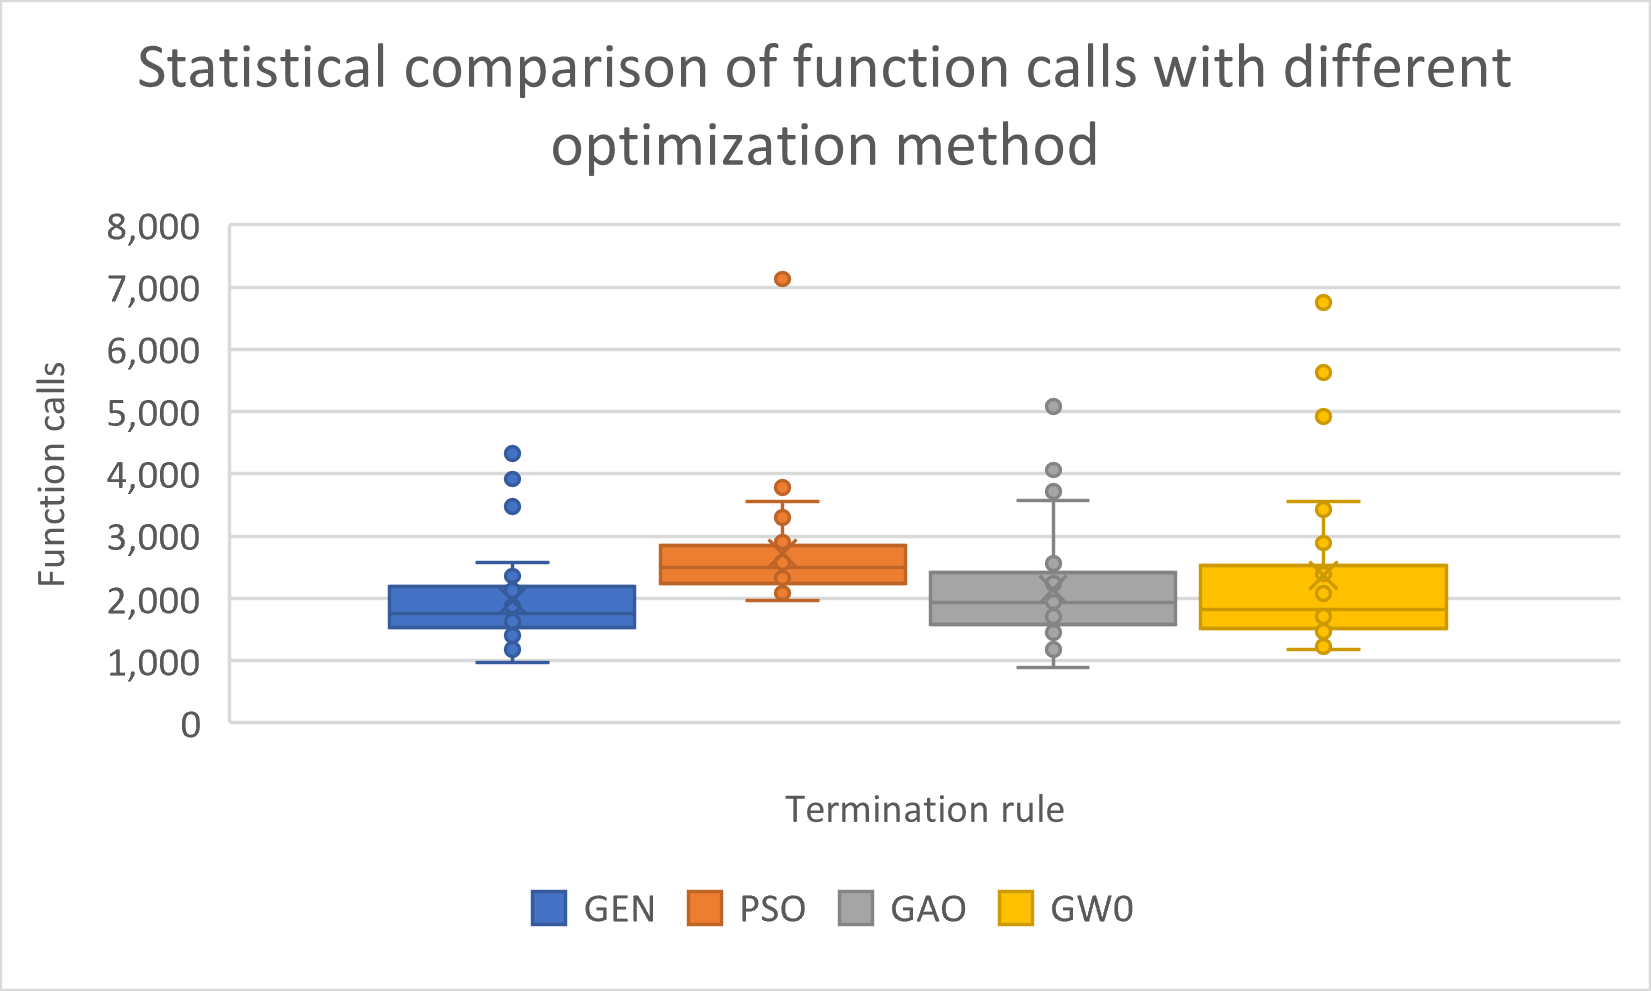
\includegraphics[scale=0.95]{gao_calls.png}
\caption{A statistical comparison using the number of function  calls. The test was performed for  three different optimization methods. \label{fig:methods}}
\end{figure}

The reliability of the termination techniques was tested with one more experiment, in which both proposed termination rules were used, and the produced results for the benchmark functions are presented in Table \ref{tab:termination}. Also, the statistical comparison for the experiment is shown graphically in Figure \ref{fig:twoStop}.

\begin{table}[H]
\caption{ Average number of function calls for the proposed method using the two suggested termination rules.\label{tab:termination}}
\begin{center}
    \begin{tabular}{|c|c|c|}
    \toprule 
\textbf{PROBLEM
} & \textbf{Similarity} & 
\textbf{Doublebox}  \tabularnewline
\hline
BF1 & 2239 & 2604 \tabularnewline
\hline
BF2	& 1974 & 1864
\tabularnewline
\hline
BRANIN 	& 1179	& 1179\tabularnewline
\hline
CAMEL &	1450 & 1245 	\tabularnewline
\hline
EASOM &	886	&	775 
\tabularnewline
\hline
EXP4 	& 1499	& 1332		
\tabularnewline
\hline
EXP8 	& 1539 & 1371		
\tabularnewline
\hline
EXP16 &	1581	&1388	
\tabularnewline
\hline
EXP32 &	1567	& 1384 	
\tabularnewline
\hline
GKLS250 	&  1292	& 1483	
\tabularnewline
\hline
GKLS350 &	1510	& 2429	
\tabularnewline
\hline
GOLDSTEIN 	& 	1953 & 2019
\tabularnewline
\hline
GRIEWANK2 &	2657  &	5426
\tabularnewline
\hline
GRIEWANK10 &		4064(0.97) & 4940 (0.97)
\tabularnewline
\hline
HANSEN &	1885	& 4482
\tabularnewline
\hline
HARTMAN3 &	1448	 & 1458 
\tabularnewline
\hline
HARTMAN6 &	1815	&	1625
\tabularnewline
\hline
POTENTIAL3 	& 1942	&	1700 
\tabularnewline
\hline
POTENTIAL5 &		3722 & 3395	
\tabularnewline
\hline
RASTRIGIN &	2411 &	4591
\tabularnewline
\hline
ROSENBROCK4 &2690 &	 2371	
\tabularnewline
\hline
ROSENBROCK8 &	3573 &	3166
\tabularnewline
\hline
ROSENBROCK16 &	5085	&	4386
 \tabularnewline
\hline
SHEKEL5 &	1911 &	1712	
\tabularnewline
\hline
SHEKEL7 &		1930 &	1722	
\tabularnewline
\hline
SHEKEL10 &		1952 &	1956	
 \tabularnewline
\hline
TEST2N4 &	1840(0.83)	&	3103(0.83)
\tabularnewline
\hline
TEST2N5 &	2029(0.63) &	3375(0.67)
\tabularnewline
\hline
TEST2N6 &	2438(0.80)	&	4458(0.83)
\tabularnewline
\hline
TEST2N7	&  2567(0.60)	&	4425(0.63)
\tabularnewline
\hline
SINU4 &	1712 &	 1657 
\tabularnewline
\hline
SINU8 &	1992	&	1874 
\tabularnewline
\hline
SINU16 	& 2557	&	2612	
\tabularnewline
\hline
TEST30N3 	& 1749 &	 1483	
 \tabularnewline
\hline
TEST30N4  &	2344	&	2737
 \tabularnewline
\hline
\textbf{SUM}  &	74982(0.97)	&	87727(0.97)
\tabularnewline
\hline
\end{tabular}
\end{center}
\end{table}

\begin{figure}[H]

\hspace{-5pt}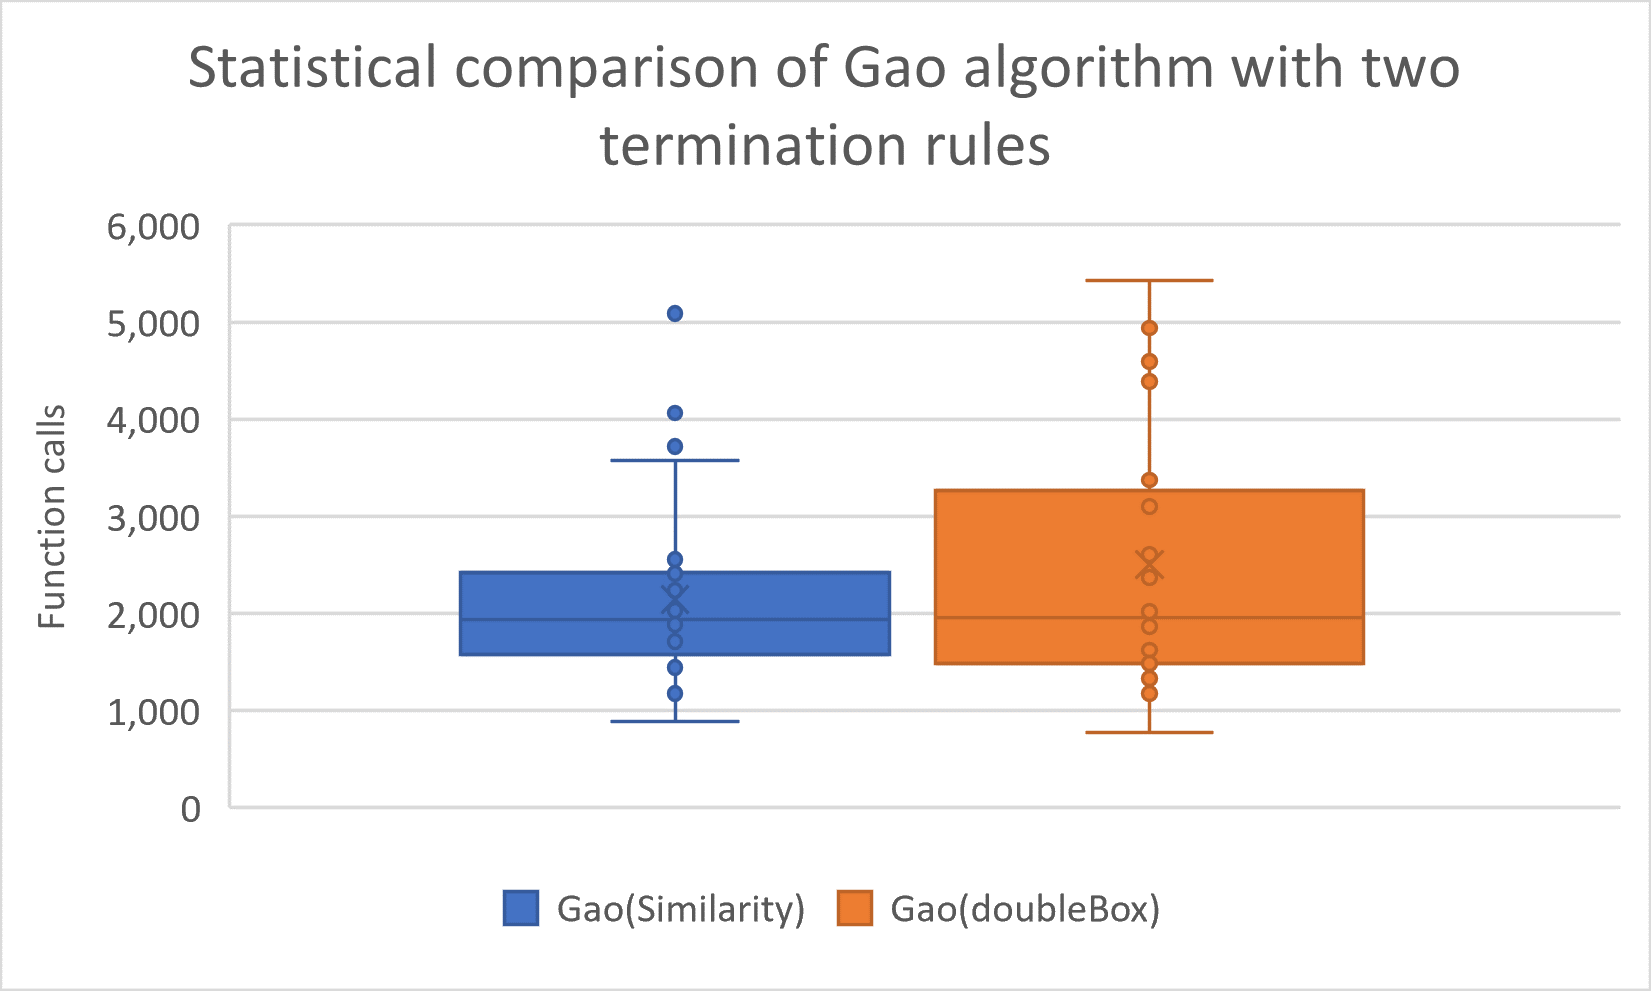
\includegraphics[scale=0.95]{gao_termination.png}
\caption{Comparison of Gao algorithm with two termination rules. \label{fig:twoStop}}
\end{figure}

From the statistical processing of the experimental results, one can find that the termination method using the \textit{Similarity} criterion demands a lower number of function calls than \textit{DoubleBox} stopping rule to achieve the goal, which is to effectively find the global minimum. Furthermore, there is no significant difference in the success rate of the two termination techniques as reflected in the success rate in finding the global minimum, which rate remains high for both techniques (around 97\%).


Moreover, the effect of the  application of the local search technique is explored in the experiments shown in Table \ref{tab:lrate}, where the local search rate increases from 0.5\% to 5\%. 
\begin{table}[H]
\caption{ Experimental results using different values for the local search rate and the proposed method.\label{tab:lrate}} 
\begin{center}
    \begin{tabular}{|c|c|c|c|}
    \hline 
\textbf{PROBLEM
} & $p_l=0.005$ & 
$p_l=0.01$ & 
$p_l=0.05$ \tabularnewline
    \hline 
BF1 & 1531 (0.97) & 1559 & 2239 \tabularnewline
    \hline 
BF2	& 1457 (0.97)	& 1319	& 1864
\tabularnewline
    \hline 
BRANIN 	& 921	& 913	& 	1179\tabularnewline
    \hline 
CAMEL &	1037 & 1022	& 1450 	\tabularnewline
    \hline 
EASOM &	871 & 850	&	886 
\tabularnewline
    \hline 
EXP4 	& 942	& 926	& 1499		
\tabularnewline
    \hline 
EXP8 	& 930 & 936 & 1539		
\tabularnewline
    \hline 
EXP16 &	1020	& 961	&1581	
\tabularnewline
    \hline 
EXP32 &	1005 & 982	& 1567 	
\tabularnewline
    \hline 
GKLS250 	&  1197 & 1106	& 	1292	
\tabularnewline
    \hline 
GKLS350 &	1256	& 1221 & 1510	
\tabularnewline
    \hline 
GOLDSTEIN 	& 	1124 & 1146& 1953
\tabularnewline
    \hline 
GRIEWANK2 &	1900 (0.93)	& 1976(0.97) &	2657
\tabularnewline
    \hline 
GRIEWANK10 &		1444(0.40)	& 1963(0.70) & 4064 (0.97)
\tabularnewline
    \hline 
HANSEN &	1872 &	1726(0.93)	& 1885
\tabularnewline
    \hline 
HARTMAN3 &	1005 & 967	 & 1448 
\tabularnewline
    \hline 
HARTMAN6 &	976(0.87)	&	1052(0.97)	&	1815
\tabularnewline
    \hline 
POTENTIAL3 	& 1018 & 1081	&	1942 
\tabularnewline
    \hline 
POTENTIAL5 &		1313	& 1439 & 3722	
\tabularnewline
    \hline 
RASTRIGIN &	1614(0.97) 	&	1687(0.97) &	2411
\tabularnewline
    \hline 
ROSENBROCK4 &	1097 & 1203 &	 2690	
\tabularnewline
    \hline 

ROSENBROCK8 &	1179	& 1403 &	3573
 \tabularnewline
    \hline 
ROSENBROCK16 &	1437 & 1801	&	5085
\tabularnewline
    \hline 
SHEKEL5 &	1070(0.97)	&	1073 &	1911	
\tabularnewline
    \hline 
SHEKEL7 &		1076(0.93)	 & 1124 &	1930	
 \tabularnewline
    \hline 
SHEKEL10 &		1152(0.97) & 1170(0.97) &	1952	
\tabularnewline
    \hline 
TEST2N4 &	1409(0.80) &	1285(0.87)	&	1840(0.83)
 \tabularnewline
    \hline 
TEST2N5 &	1451(0.53)	&	1350(0.63) &	2029(0.63)
\tabularnewline
    \hline 
TEST2N6 &	1417(0.60) &	1529(0.67)	&	2438(0.80)
\tabularnewline
    \hline 
TEST2N7	&  1500 (0.47) & 1451(0.33)	&	2567(0.60)
\tabularnewline
    \hline 
SINU4 &	1210 & 1199 &	 1712 
\tabularnewline
    \hline 
SINU8 &	1163 & 1145	&	1992 
 \tabularnewline
    \hline 
SINU16 	& 1377 	&	1296 &	2557	
\tabularnewline
    \hline 
TEST30N3 	& 1057 & 1189 &	 1749	
 \tabularnewline
    \hline 
TEST30N4  &	1897  & 3817	&	2344
\tabularnewline
    \hline 
\textbf{SUM}  &	43213(0.92)	&	44331(0.94)	&	74982(0.97)
\tabularnewline
    \hline 
\end{tabular}
\end{center}
\end{table}
As it was expected, the success rate in discovering the global minimum increases as the rate of application of the local minimization technique increases. For the case of the current method this rate increases from 92\% to 97\% in the experimental results. This finding demonstrates that if this method is combined with effective local minimization techniques, it can lead to more efficient finding of the global minimum for the objective function.

Also, in order to measure the time complexity of the proposed work the ELP (High Elliptic Function) function was employed with arbitrary dimension. The function is defined as:
\[
f(x)=\sum_{i=1}^{n}\left(10^{6}\right)^{\frac{i-1}{n-1}}x_{i}^{2}
\]
In this test, the dimension of the function ($n$) increased from 1 to 15 and the average execution time was measured. The results obtained for the similarity termination rule are outlined in Figure 
\ref{fig:timeSim} and the results for the doublebox termination rule are graphically shown in Figure \ref{fig:timeDouble}.

\begin{figure}[H]
\hspace{-5pt}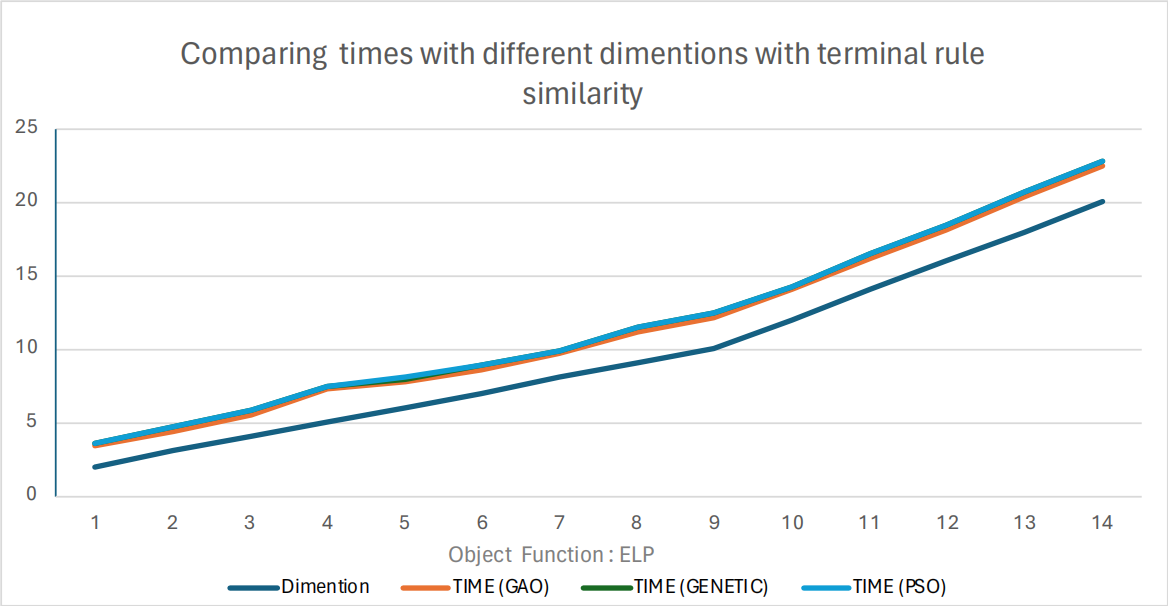
\includegraphics[scale=0.5]{time_similarity.png}
\caption{Representation of the average execution times for the ELP objective function, using the similarity stopping rule. \label{fig:timeSim}}
\end{figure}

\begin{figure}[H]
\hspace{-5pt}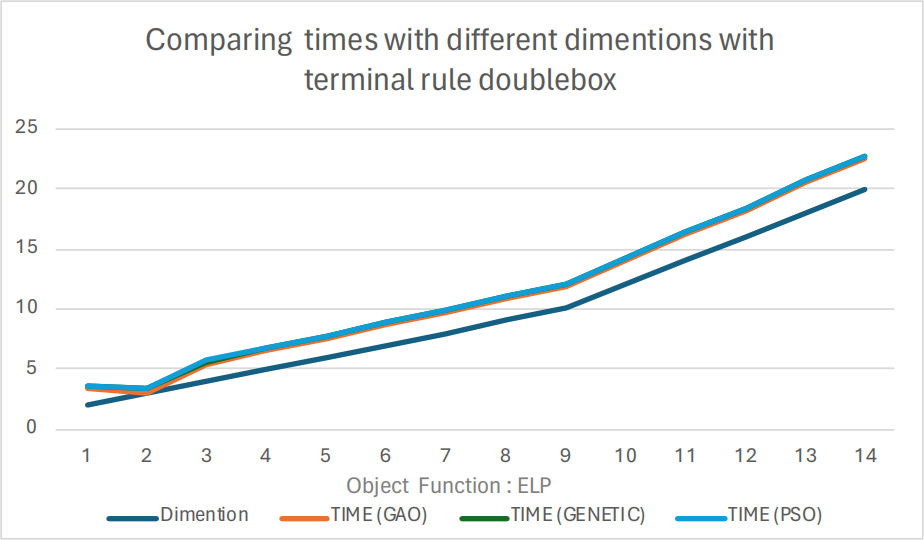
\includegraphics[scale=0.5]{time_doublebox.png}
\caption{Representation of the  average execution times for the ELP objective function, using the doublebox stopping rule. \label{fig:timeDouble}}
\end{figure}
As it was expected, the execution time increases as the dimension of the function increases but there are not significant differences between the execution times of the three optimization methods.

Furthermore, as a practical application consider the training of an artificial neural network for classification or data fitting problems \cite{ann1,ann2}.  Neural networks are non - linear parametric tools with many applications in real - world problems \cite{ann_agri,ann_facial,ann_physics}.
Neural networks can be defined as a functions \textbf{$N(\overrightarrow{x},\overrightarrow{w})$
}. The vector $\overrightarrow{x}$ represents the input pattern
while the vector \textbf{$\overrightarrow{w}$ }represents  the weight vector of the neural network, that should be estimated.
Optimization methods can be used to estimate the set of weights by minimizing the following
equation:

\begin{equation}
E\left(N\left(\overrightarrow{x},\overrightarrow{w}\right)\right)=\sum_{i=1}^{M}\left(N\left(\overrightarrow{x}_{i},\overrightarrow{w}\right)-y_{i}\right)^{2}\label{eq:eqN}
\end{equation}
The quantity of Equation \ref{eq:eqN} was minimized using the mentioned algorithm of this work for the BK dataset \cite{bk_problem}, that is used  estimated the points  in a basketball game. The average test error using the four methods presented in this article is shown graphically in figure \ref{fig:mlpTest}. To validate the results the well - known method of ten - fold cross was applied. The current work has the same performance as the PSO algorithm and outperforms significantly the Genetic algorithm.
\begin{figure}[H]
\hspace{-5pt}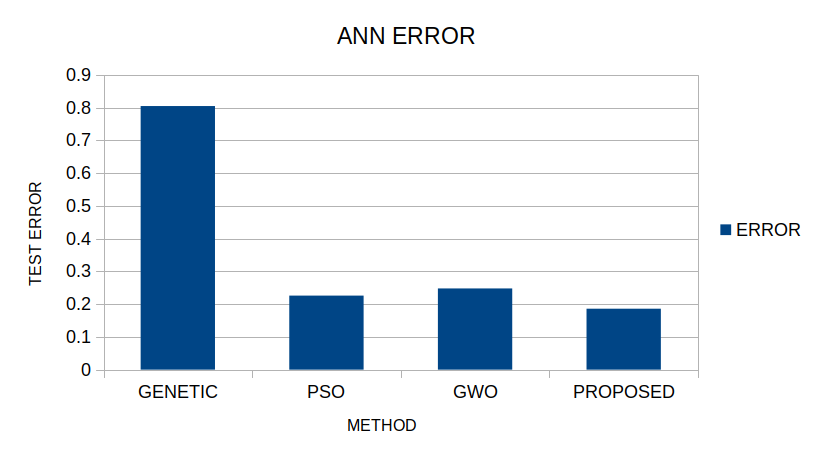
\includegraphics[scale=0.5]{mlp_test.png}
\caption{Comparison of test error between the mentioned global optimization algorithms for the BK dataset. \label{fig:mlpTest}}
\end{figure}
\section{Conclusions}\label{sec:Conclusions}
Two modifications for the Giant Armadillo Optimization method was suggested in this article. These modifications aimed to improve the efficiency and the speed of the underlying global optimization algorithm. The first modification suggested the periodically application of a local optimization procedure to randomly selected armadillos from the current population. The second modification utilized some stopping rules from the recent bibliography in order to stop more efficient the optimization method and to avoid  unnecessary iterations, when the global minimum was already discovered. The modified global optimization method was tested against two other global optimization methods from the relevant literature and more specific an implementation of the Genetic Algorithm and a Particle Swarm Optimization variant on a series of well - known test functions. In order to have a fair comparison between these methods, the same number of test solutions (armadillo or chromosomes) as well as the same termination rule were used. The present technique after comparing the experimental results shows that it clearly outperforms the particle optimization and has similar behavior to that of the genetic algorithm. Also, after a series of experiments it was shown that the Similarity termination rule outperforms the DoubleBox termination rule in terms of function calls, without reducing the effectiveness of the proposed  method in the task of locating the global minimum.

Since the experimental results show to be extremely promising further efforts can be made for the development of the technique in various fields.  For example, an extension could be to develop a termination rule that exploits the particularities of the particular global optimization technique.
 Among the future extensions of the application may be the use of parallel computing techniques to speed up the optimization process, such as the incorporation of the MPI  \cite{openmpi}  or the  OpenMP library \cite{openmp}. For example, in this direction it could be investigated to parallelize the technique in a similar way as genetic algorithms using islands \cite{island1,island2}.\vspace{6pt} 

\authorcontributions{G.K., V.C. and I.G.T. conceived of the idea and the methodology and G.K. and V.C. implemented the corresponding software. G.K. conducted the experiments, employing objective functions as test cases, and provided the comparative experiments. I.G.T. performed the necessary statistical tests. All authors have read and agreed to the published version of the manuscript.}

\funding{This research received no external funding.}

\institutionalreview{Not applicable.}

\informedconsent{Not applicable.}

\dataavailability{Not applicable.} 


\acknowledgments{This research has been financed by the European Union : Next Generation EU through the Program Greece 2.0 National Recovery and Resilience Plan , under the call RESEARCH – CREATE – INNOVATE, project name “iCREW: Intelligent small craft simulator for advanced crew training using Virtual Reality techniques" (project code:TAEDK-06195)}

\conflictsofinterest{The authors declare no conflicts of interest.} 



%%%%%
\begin{adjustwidth}{-\extralength}{0cm}
%\printendnotes[custom] % Un-comment to print a list of endnotes

\reftitle{References}

% Please provide either the correct journal abbreviation (e.g. according to the “List of Title Word Abbreviations” http://www.issn.org/services/online-services/access-to-the-ltwa/) or the full name of the journal.
% Citations and References in Supplementary files are permitted provided that they also appear in the reference list here. 

%=====================================
% References, variant A: external bibliography
%=====================================
%\bibliography{your_external_BibTeX_file}

%=====================================
% References, variant B: internal bibliography
%=====================================
\bibliography{bibliography}
\PublishersNote{}
\end{adjustwidth}
\end{document}

